\subchapter{Building Linux with Buildroot}{Download the Buildroot simple build system}

\section{Installing Buildroot}

For the this lab, you will build a complete distribution

{\small
{\tt
\$ cd\\
\$ mkdir -p projects/labs\\
\$ cd projects/labs\\
\$ git clone git://git.buildroot.net/buildroot\\
}
}

The buildroot system is now available in an \code{projects/labs/buildroot} directory
under your home directory.

\section{Getting the Tarballs}

Normally, Buildroot will download automatically from Internet all source tarballs needed
to build the toolchain, the kernel and the filesystem, but this can be a substantial amount, so instead  we are going to copy most of the stuff directly into the \code{dl} download directory.

{\small
{\tt
\$ cd\\
\$ mkdir -p dl\\
\$ rsync -avu <your download source> dl\\
}
}

You are now ready to start the real practical labs!

\section{Setting up Buildroot}

First you need to setup Buildroot for building the Beaglebone.
Buildroot is using the same configurationsystem as Linux (KConfig),
so you can use:

{\small
{\tt
\$ make menuconfig\\
}
}

to create a ".config" file which is used to determine what Buildroot
is going to build.

Advanced users may want to use

{\small
{\tt
\$ make xconfig\&\\
}
}

but this may need extra packages which may or may not be present on your machine.

There are a lot of options to select from, but to make it easy, someone has already
prepared a configuration which suites the Beaglebone Black and is easy to use.

{\small
{\tt
\$ make beaglebone\_defconfig\\
}
}
Now you can use the \code{make menuconfig} or \code{make xconfig&} to
make modifikations. But this will not be done right now.
We will just build the first project

{\small
{\tt
\$ make
}
}

\section{Build Times}

Alternatively, You can measure the time by using \code{time}

{\small
{\tt
\$ time make
}
}

The result for a build on a pretty nice machine \code{Core-i7 980X} (6 Cores at 3.33GHz) was.
{\small
{\tt
\begin{verbatim}
real	137m57.224s
user	42m46.980s
sys	3m23.353s
\end{verbatim}
}
}
During that time, Buildroot downloaded 23 tarballs from Internet, totalling 324,6 MB
and created 196 406 objects in the \code{output} directory, totalling about 3,5 GB.

To test the performance of a buoild with the tarballs already in place, the \code{output} directory was deleted, \code{Don't do that!} and the system was again built, now with
the tarballs already available in the \code{dl} directory

The result of this was much more encouraging.
{\small
{\tt
\begin{verbatim}
real	16m9.196s
user	40m10.307s
sys	3m12.252s
\end{verbatim}
}
}

\section{Build Results}

At the end of the build, you will have 5 files located in \code{output/images}.

\begin{itemize}

\item MLO

\item u-boot.img

\item uImage

\item am335x-bone.dtb

\item rootfs.ext2

\end{itemize}

\section{Booting the Beaglebone}

The Beaglebone has a Texas Instruments \code{AM3359 Sitara} processor onboard.
It is based on an \code{ARMv7} architecture.

When the processor is reset, it will read a second level bootloader \code{MLO} from a boot source defined by the state of some I/O pins during reset.

On expensive development boards there are typically switches to allow easy selection of the boot source from a multitude of choices.

The Beaglebone Black will always boot from the on board eMMC memory unless button S2 is pressed,
in which case it will boot from the microSD card we plan to use.

MLO will initialize the memory subsystem and load the main bootloader U-Boot from u-boot.img.

U-Boot can be configured through it environment variable.

Two important U-Boot variables are \code{bootcmd} and \code{bootargs}.
If the board is left to itself, it will "run" the \code{bootcmd},
which will normally load the linux kernel and execute it,
with \code{bootargs} passed to the kernel.

Even though the beaglebone default configuration is to boot from internal memory (eMMC),
the predefined U-Boot environment will try to boot from the SD-Card so normally
the button S2 does not need to be pressed.

The SD-Card needs to formatted into two partitions, and this will be described in another chapter.

\begin{itemize}

\item Partition 1: FAT32 formatted

\item Partition 2: EXT4 formatted

\end{itemize}


U-Boot will first try to load the file \code{"uEnv.txt"} from the FAT32 partition,
and update its internal environment.
Unless the file updates certain environment variables,
U-Boot will continue and load the kernel \code{"uImage"} and a \code{"device tree file"}
from the second partition. Both are located inside the \code{"boot"} subdirectory which
needs to be an \code{ext4} file system.

Buildroot will not generate the uEnv.txt file but example files
can be found on Internet and one will be provided.

The device-tree concept is relatively new to the ARM linux ecosystem.
It has been around for some time for PowerPC processors. The device tree file
is loaded by the kernel at boot time and is used to determine which peripheral drivers
to load and in which order. Two different chips can therefore boot with the same kernel
but with different device files.


\section{Problems with the Buildroot build}

The results of the buildroot build is really not useful in the current state.

First of all, since the Beaglebone Black will be using the MLO and u-boot.img
on the eMMC card, they are not needed (at least for the training).

Since U-Boot will read the kernel (uImage) and device file (am335x-bone.dtb)
from the file system the separate kernel and device file will also not be needed.

Only the file system file (rootfs.ext2) will be needed.
An observant reader will have noted another problem.
The standard configuration will generate an ext2 filesystem,
and we want to have an ext4 filesystem.

The normal way of generating an SD card file system is not to
copy a binary filesystem like rootfs.ext2 to the SD-Card.
Instead the an empty filesystem is created on the SD-Card,
and then a tarball containing the filesystem is unpacked on top.

Buildroot does not generate the tarball right now, but it can be configured to do so.

Once the tarball is generated, a quick inspection will reveal further problems.
There is no \code{/boot} directory, and thus there is no kernel or device file.

This can be solved by changing the U-Boot environment variables to
load them from the SD-Card but we can solve it at least partially
with Buildroot.

Once we have a filesystem in a tarball with the kernel and device file we could
generate a an SD-Card and try to boot. The boot will fail, because U-Boot will
look for \code{"am335x-boneblack.dtb"} but Buildroot generated \code{"am335x-bone.dtb"}
which is the device file for the standard Beaglebone and not the Beaglebone Black.


\section{Fixing the problems}

From the buildroot top directory \code{projects/labs/buildroot} we will
change the Buildroot configuration

{\small
{\tt
\$ make menuconfig
}
}

The configuration application is built and executed and you will get
the following window:

\begin{center}
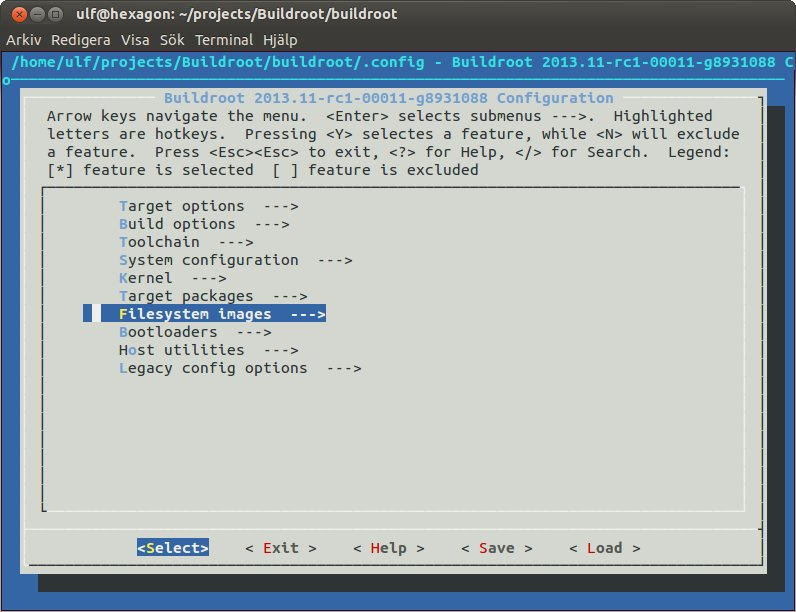
\includegraphics[width=14cm]{labs/buildroot/menuconfig_top.jpg}
\end{center}

First will we make sure that the correct image is built,
so use the arrow buttons to move down the cursor to "Filesystem Images"
and select with the \textless RETURN\textgreater button.


\clearpage
This will change the view to:

\begin{center}
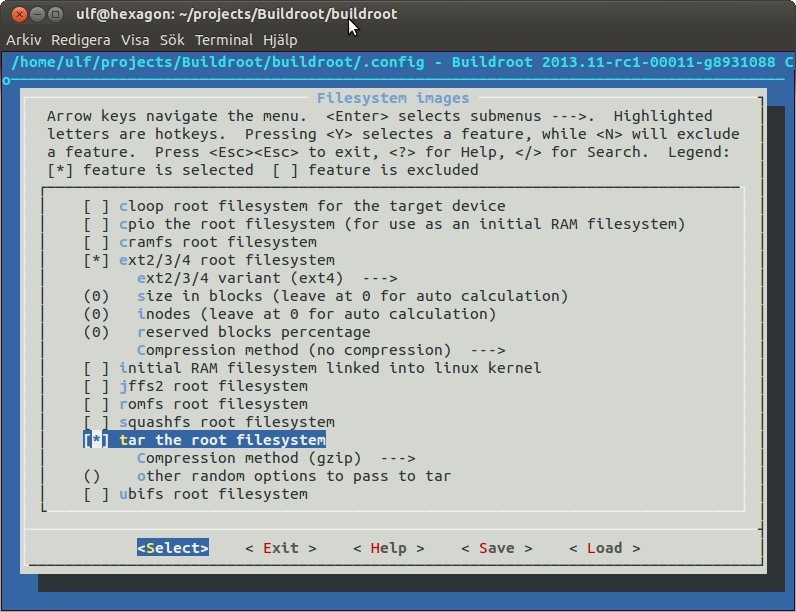
\includegraphics[width=14cm]{labs/buildroot/menuconfig_tar_gz.jpg}
\end{center}

You need to do two changes here.

Change the ext2/ext3/ext4 parameter from \code{ext2} to \code{ext4}

This is not 100\% neccessary, since will generate \code{rootfs.ext4}
which won't be used, but it might give a hint to the casual user what
Beaglebone Black expects, so we will have it enabled.

Enable the \code{tar the root filesystem} option by selecting
it with the arrow keys and then press \textless SPACE \textgreater

Select \code{gzip} as the the Compression Method. (You should now understand how)

Use the right arrow key to select  \textless EXIT \textgreater to return
to the main window.

Select the kernel subwindow and press \textless RETURN\textgreater

\clearpage
The new view will be:

\begin{center}
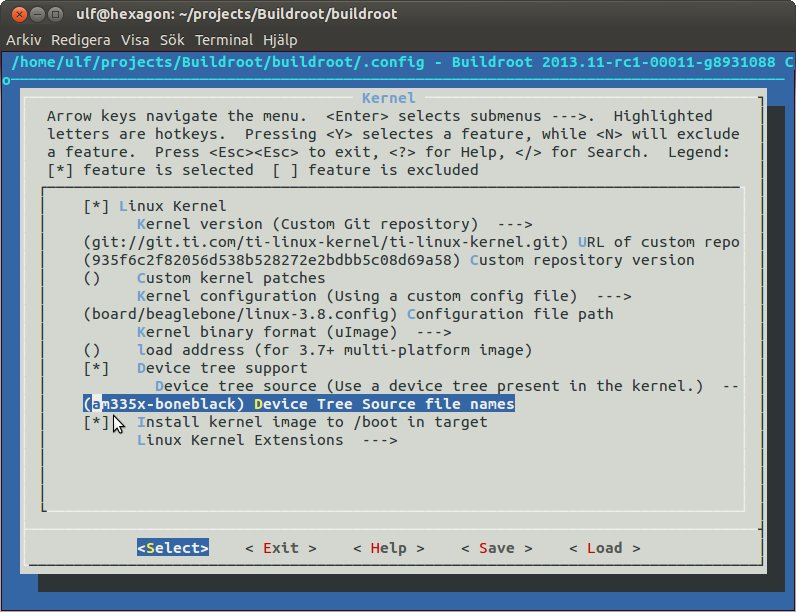
\includegraphics[width=14cm]{labs/buildroot/menuconfig_kernel.jpg}
\end{center}

Make sure you enable the \code{Install kerenl image to /boot in target} option

Also change the name of the \code{Device Tree Source file names} from
\code{am335x-bone} to \code{am335x-boneblack}.

Exit the view into the main view, and exit that as well.

Make sure the configuration is saved.

Since we have done some changes to the way the kernel should be built,
we will clean the build.


{\small
{\tt
\S \ make linux-clean
}
}

Followed by a remake of the Buildroot

{\small
{\tt
\$ make
}
}

Since we have not done that many changes, the rebuild will be quick.

We now have a few additional files in the \code{output/images} directory.
The most important is \code{rootfs.tar.gz} which contains the filesystem
in the correct format with a \code{/boot} directory containing the kernel
and device tree file.

\clearpage

Once you have a formatted SD-Card with an ext4 file system,
you make sure that the file system is mounted.
Ubuntu has an automounter which will mount the SD-Card ext4
partition on \code{/media/rootfs}

If that does not work, the manual way is:

{\small
{\tt
\$ sudo mkdir -p /media/rootfs\\
\$ sudo mount -t ext4 /dev/sd\textless n\textgreater /media/rootfs
}
}

Once you have the SD-Card mounted on \code{/media/rootfs} you can decompress
the filesystem:

{\small
{\tt
\$ sudo tar -zxvf output/images/rootfs.tar.gz -C /media/rootfs
}
}



\clearpage
\section{More guidelines}

Can be useful throughout any of the labs

\begin{itemize}

\item Read instructions and tips carefully. Lots of people make
  mistakes or waste time because they missed an explanation or a
  guideline.

\item Always read error messages carefully, in particular the first
  one which is issued. Some people stumble on very simple errors just
  because they specified a wrong file path and didn't pay enough
  attention to the corresponding error message.

\item Never stay stuck with a strange problem more than 5
  minutes. Show your problem to your colleagues or to the instructor.

\item You should only use the \code{root} user for operations that require
  super-user privileges, such as: mounting a file system, loading a
  kernel module, changing file ownership, configuring the
  network. Most regular tasks (such as downloading, extracting
  sources, compiling...) can be done as a regular user.

\item If you ran commands from a root shell by mistake, your regular
  user may no longer be able to handle the corresponding generated
  files. In this case, use the \code{chown -R} command to give the new
  files back to your regular user.\\
  Example: \code{chown -R myuser.myuser linux-3.4}

\end{itemize}
